\documentclass{article}

%%% Fill details here (in the second brackets)
\newcommand{\name}{Hao Sun}     % Your name (First Last)
\newcommand{\wustlkey}{sun.hao}             % Your WUSTL Key
%%%



%%%%%%%%%%%%%%%%%%%%%% Formatting Stuff %%%%%%%%%%%%%%%%%%%%%%%%%%%
\usepackage{times}
\usepackage[T1]{fontenc}

\setlength{\parskip}{1em}\setlength{\parindent}{0pt}
\linespread{1.25}
\usepackage[margin=0.7in,top=1in]{geometry}\usepackage{fancyhdr}
\pagestyle{fancy}\lhead{\bf \name}\rhead{\bf \wustlkey}\cfoot{\thepage}
\newcommand{\info}{\clearpage \subsection*{Information}}

\newcommand{\solution}[1]{\clearpage \subsection*{Solution #1}}  % define a new command \solution without index number
\newcommand{\spart}[1]{\paragraph{(#1)}} 
%%%%%%%%%%%%%%%%%%%%%%%%%%%%%%%%%%%%%%%%%%%%%%%%%%%%%%%%%%%%%%%%%%%


%%% Add any more packages if you want to
\usepackage{amsmath,graphicx}


\begin{document}
%%%%% Main Body goes here

% Begin solution to every problem like this.
\solution{1}

\spart{a} 
	Based on $x$, when $x>0$ we can get the following:
\begin{equation}
  	\left(x-y\right)^2 + \lambda*x
\end{equation}

when $x<0$ we can get the following:

\begin{equation}
  	\left(x-y\right)^2 - \lambda*x
\end{equation}

Based on (1) and (2), their minimum limit will be $x = y + \frac{\lambda}{2} (x<0)$, $x = y - \frac{\lambda}{2}  (x>0)$ and $x=0$. In the image, the minimum value will be determined by one of these three x value.

\spart{b} 
	denoise
\begin{figure*}[h!]
  \centering
  	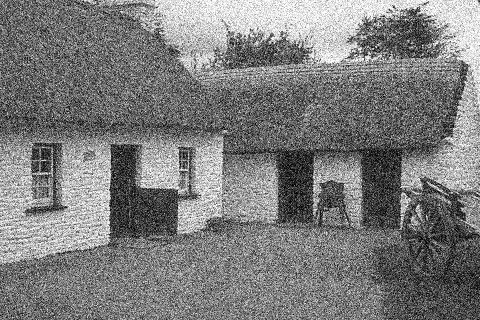
\includegraphics[height=20em]{code/inputs/p1.png}
	
\includegraphics[height=20em]{code/outputs/prob1.png}
  \caption{Denoising}
\end{figure*}

\solution{2}

\spart{a}
white balance(1)
\begin{figure*}[h!]
  \centering
  	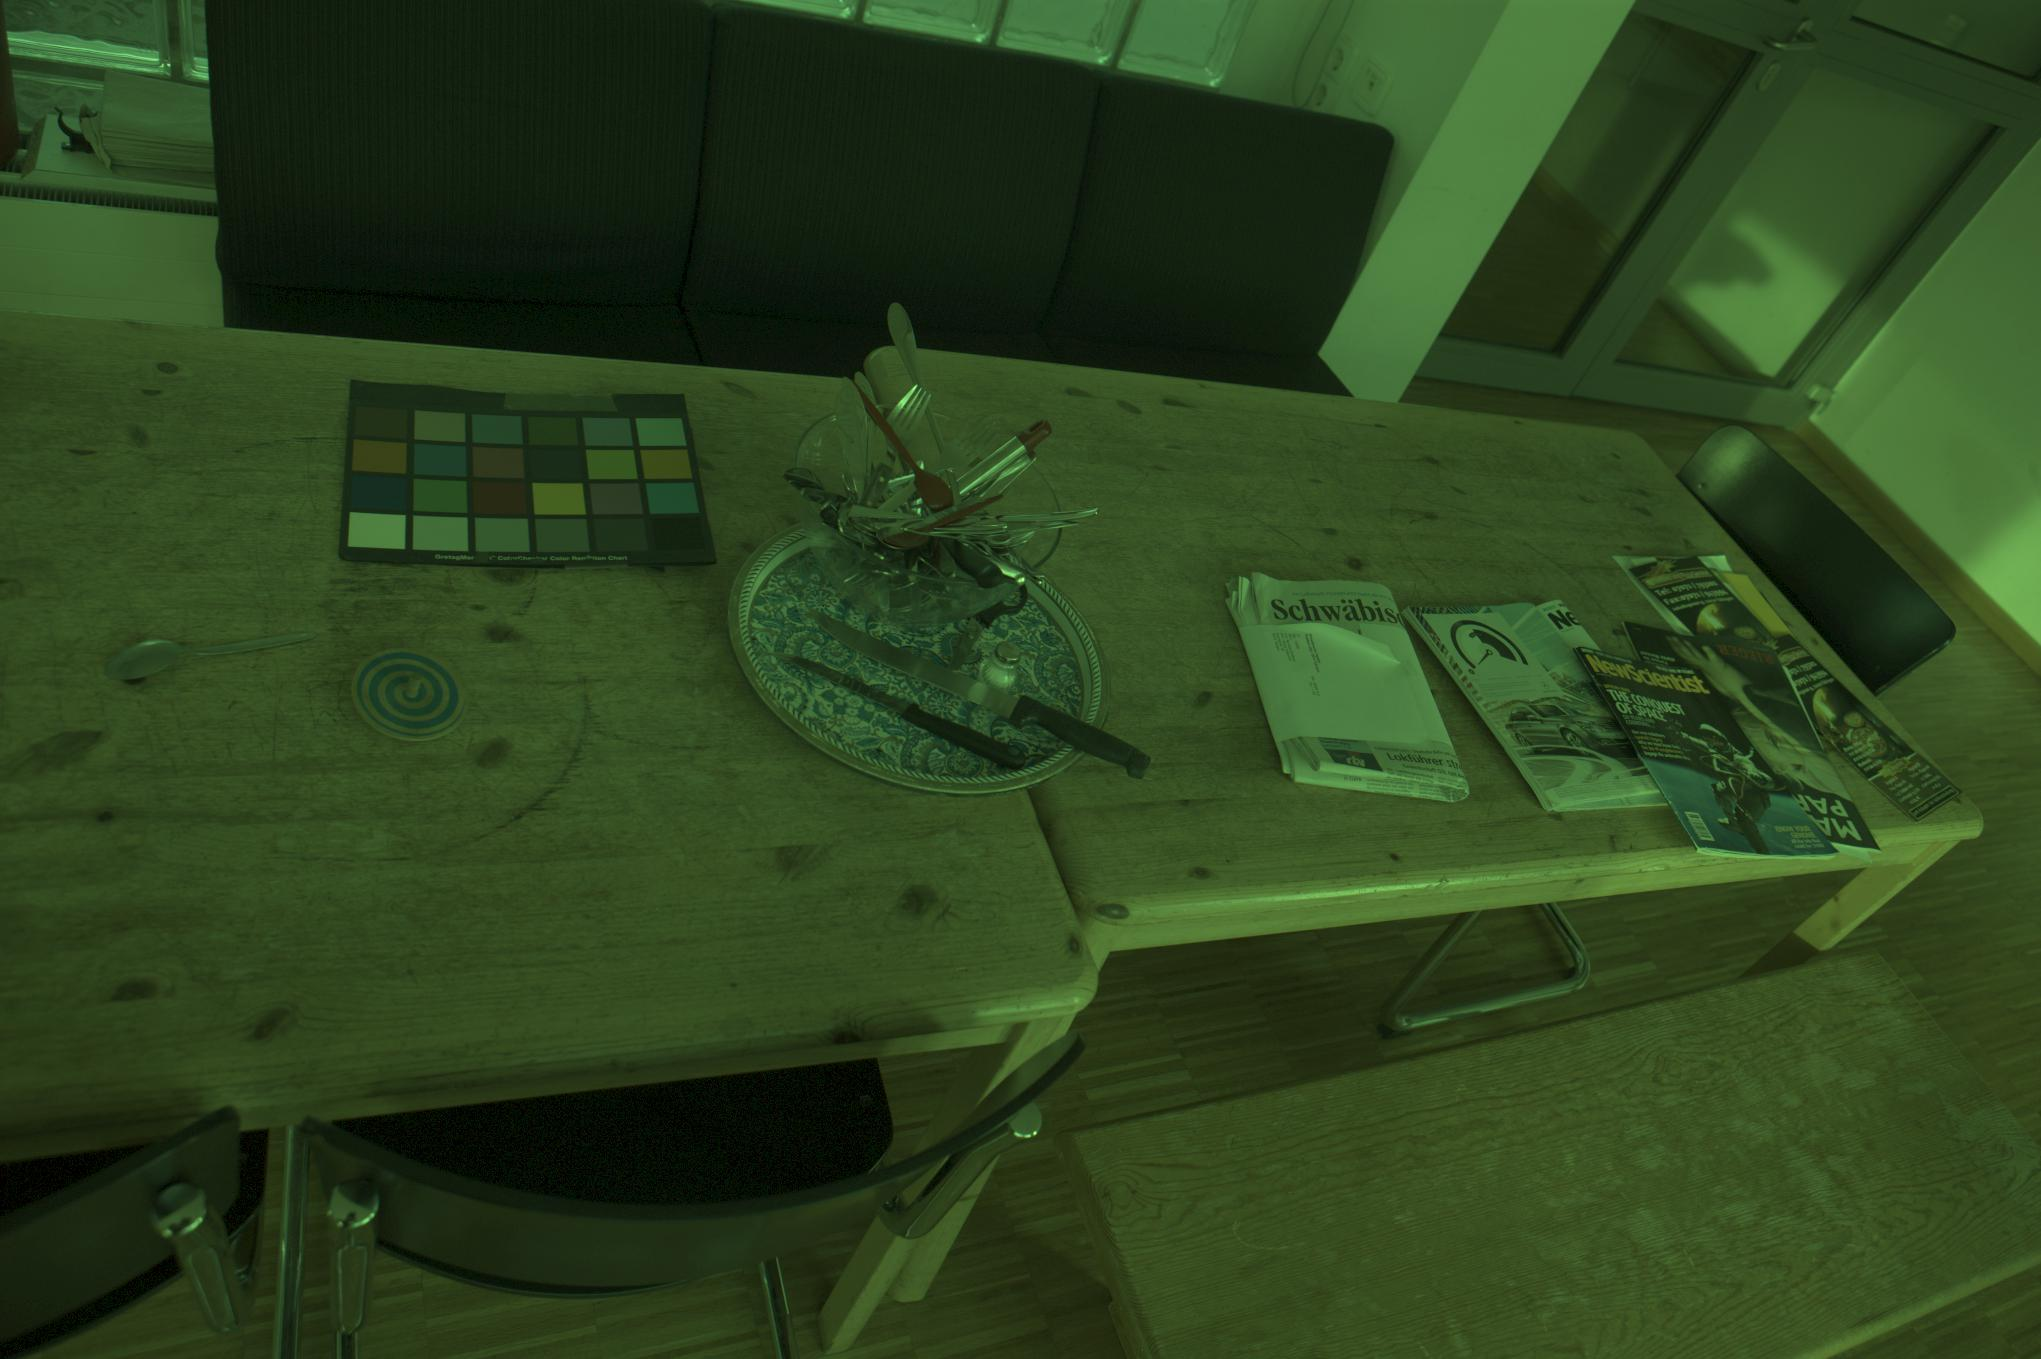
\includegraphics[height=15em]{code/inputs/cc/ex1.jpg}
	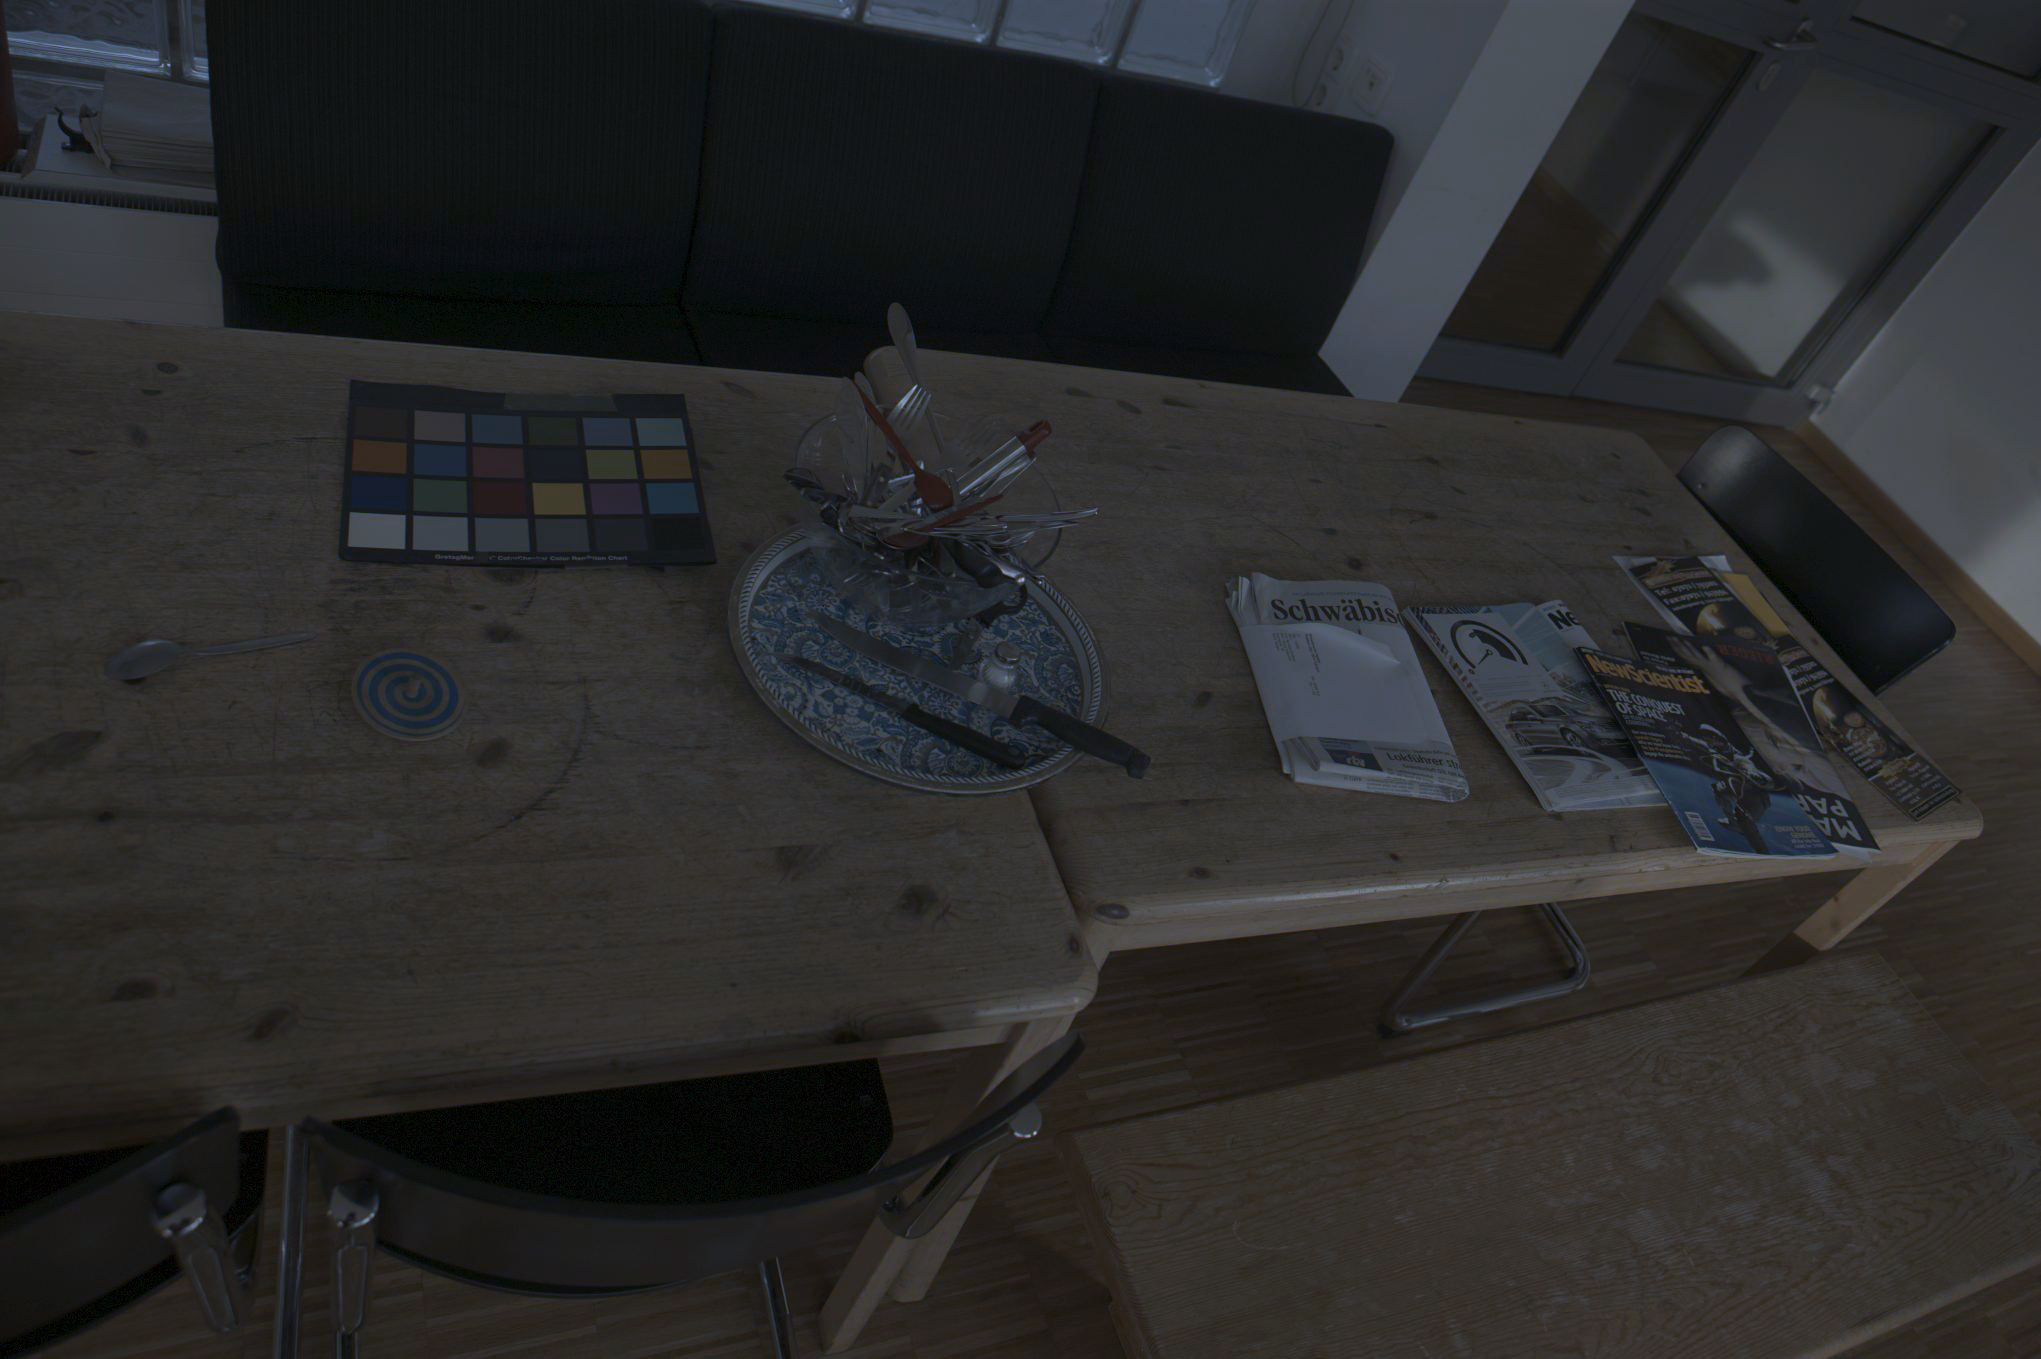
\includegraphics[height=15em]{code/outputs/prob2a_1.png}
	  \caption{balance2a-1}
\end{figure*}

\begin{figure*}[h!]
  \centering
  	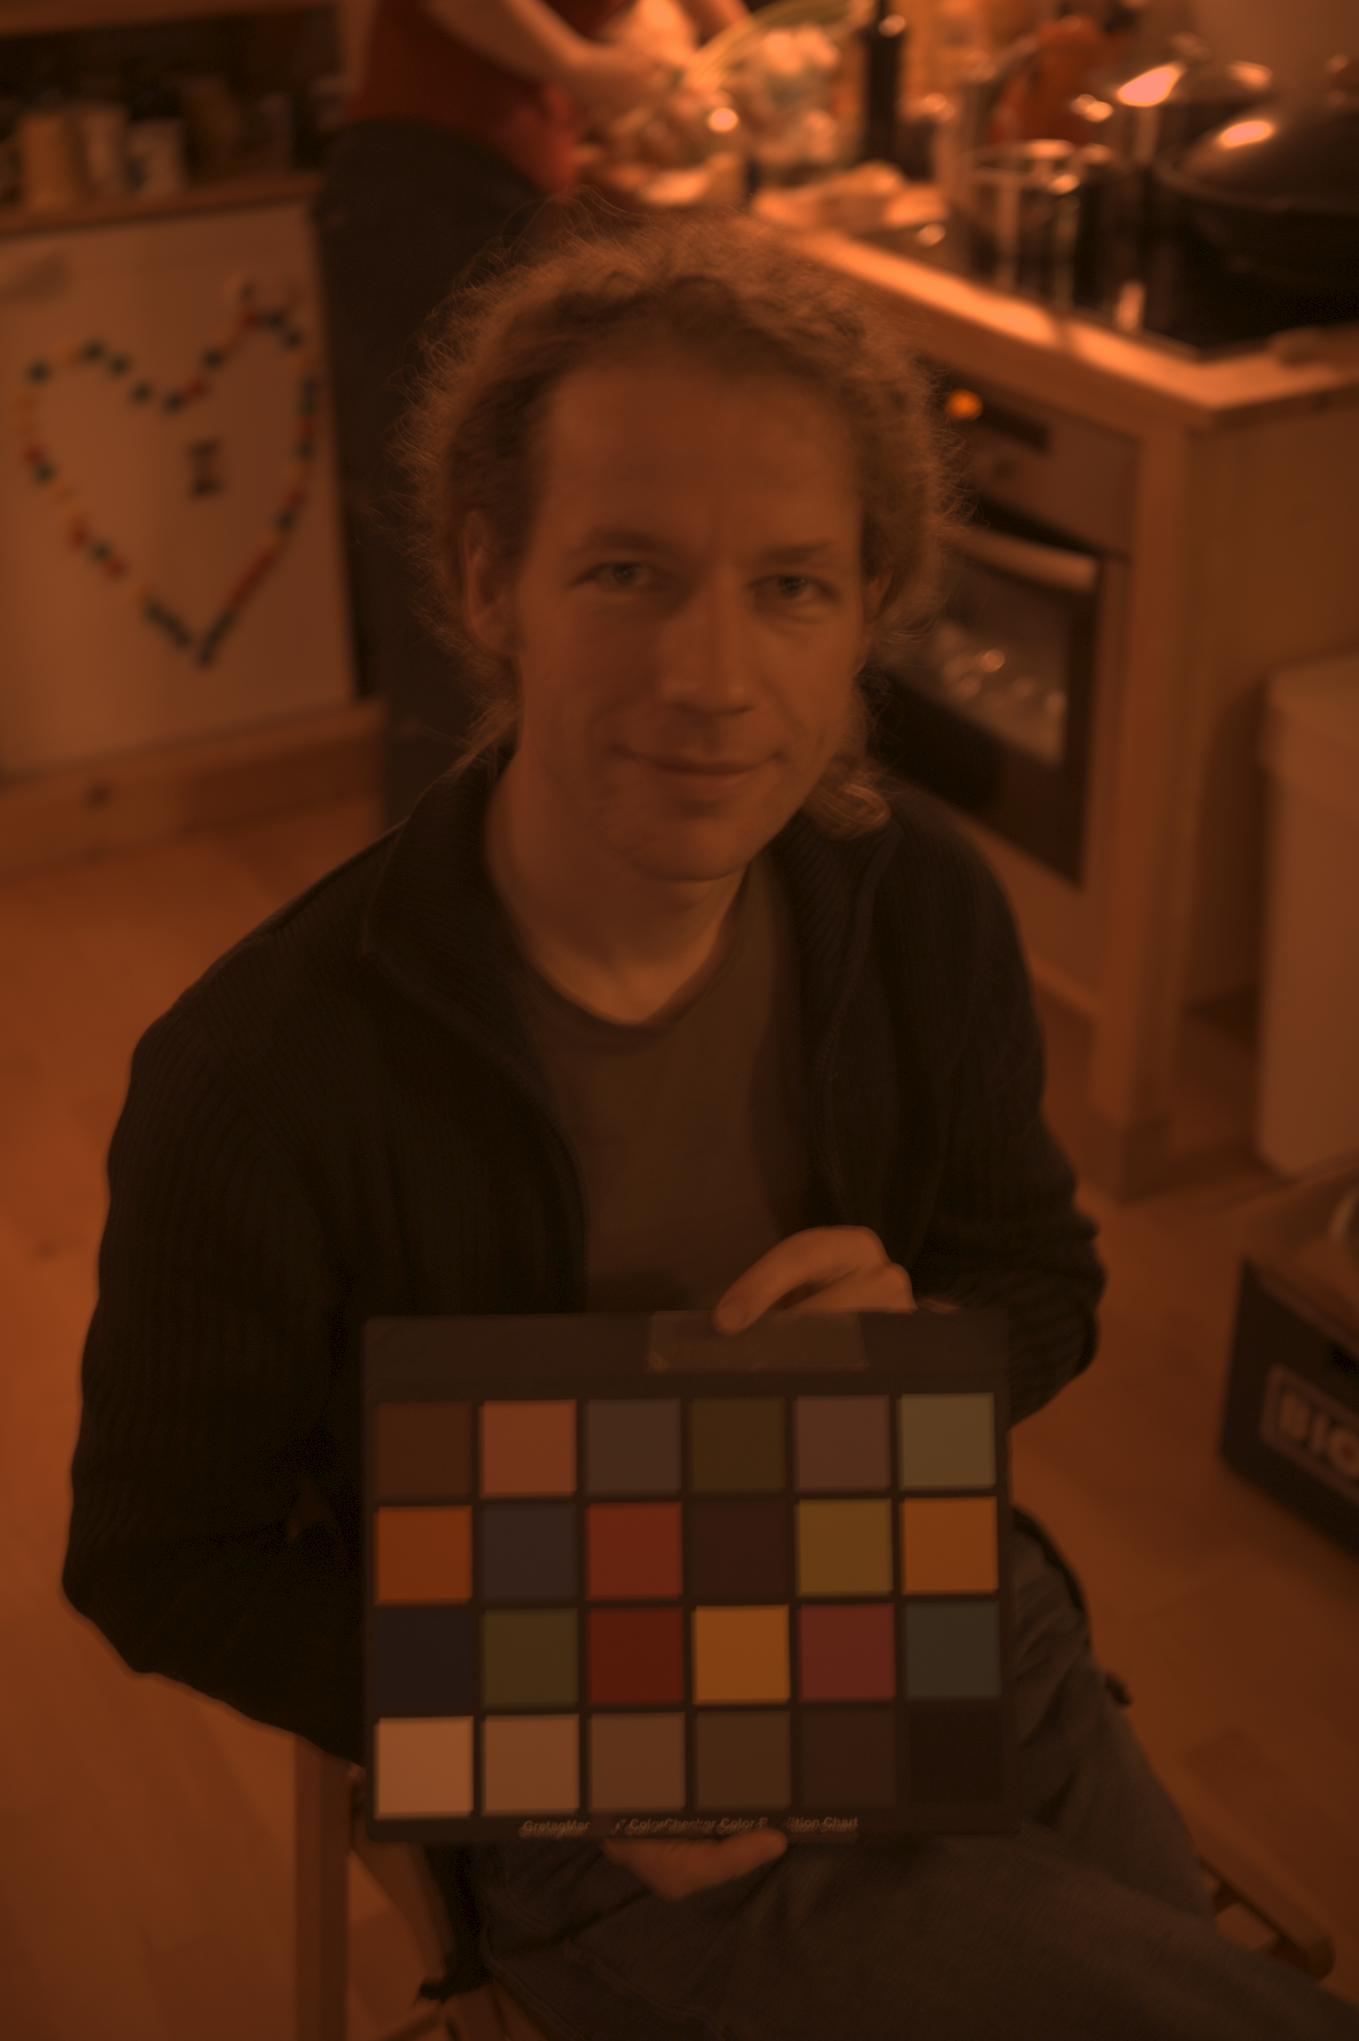
\includegraphics[height=20em]{code/inputs/cc/ex2.jpg}
	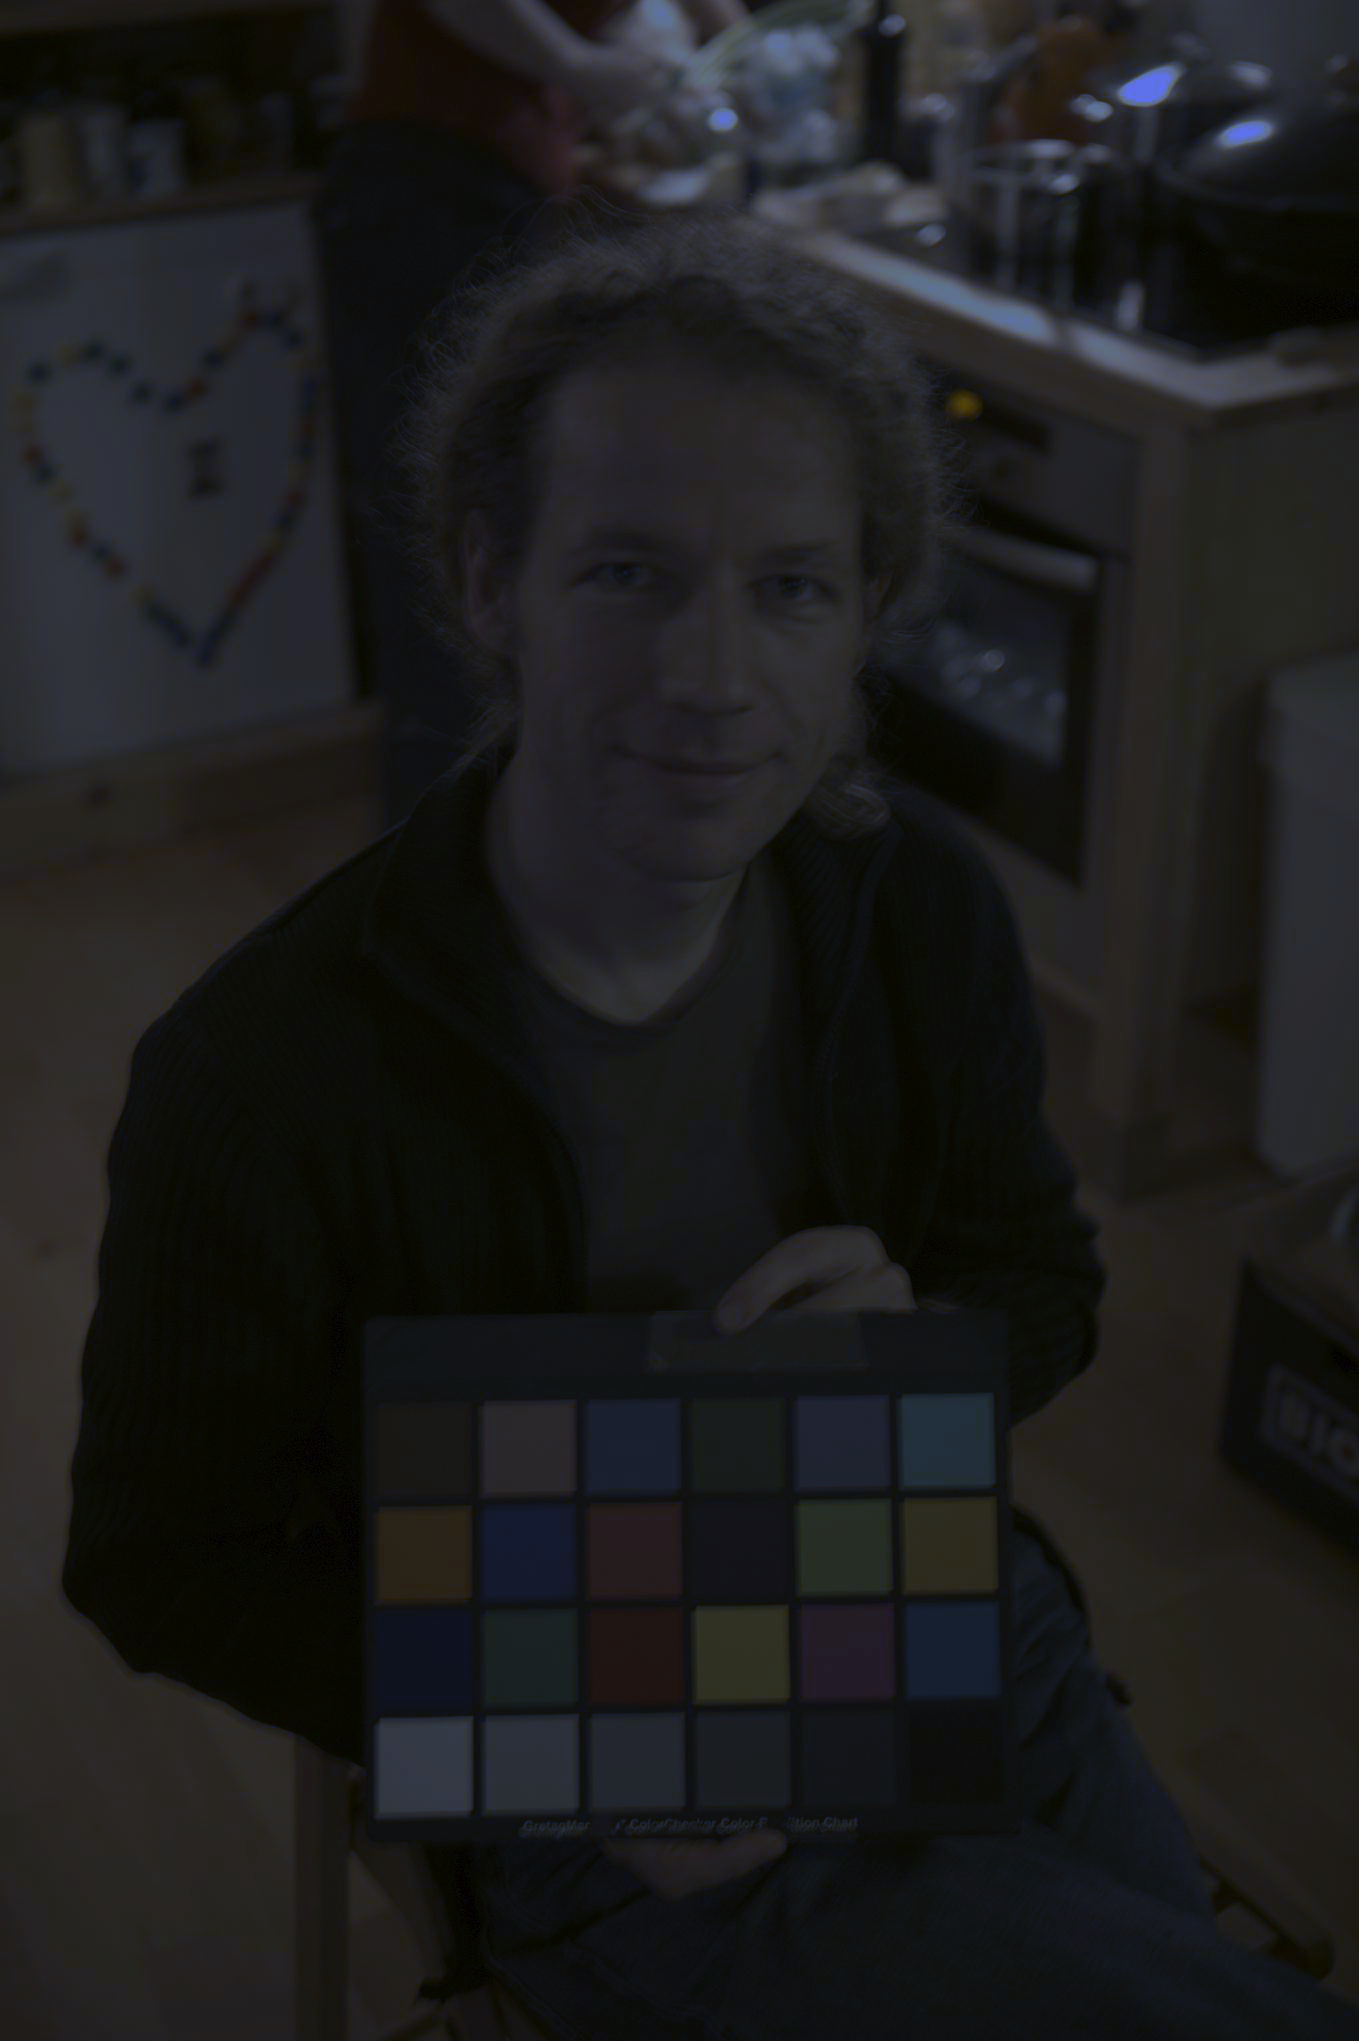
\includegraphics[height=20em]{code/outputs/prob2a_2.png}
	  \caption{balance2a-2}
\end{figure*}
\newpage

\begin{figure*}[h!]
  \centering
  	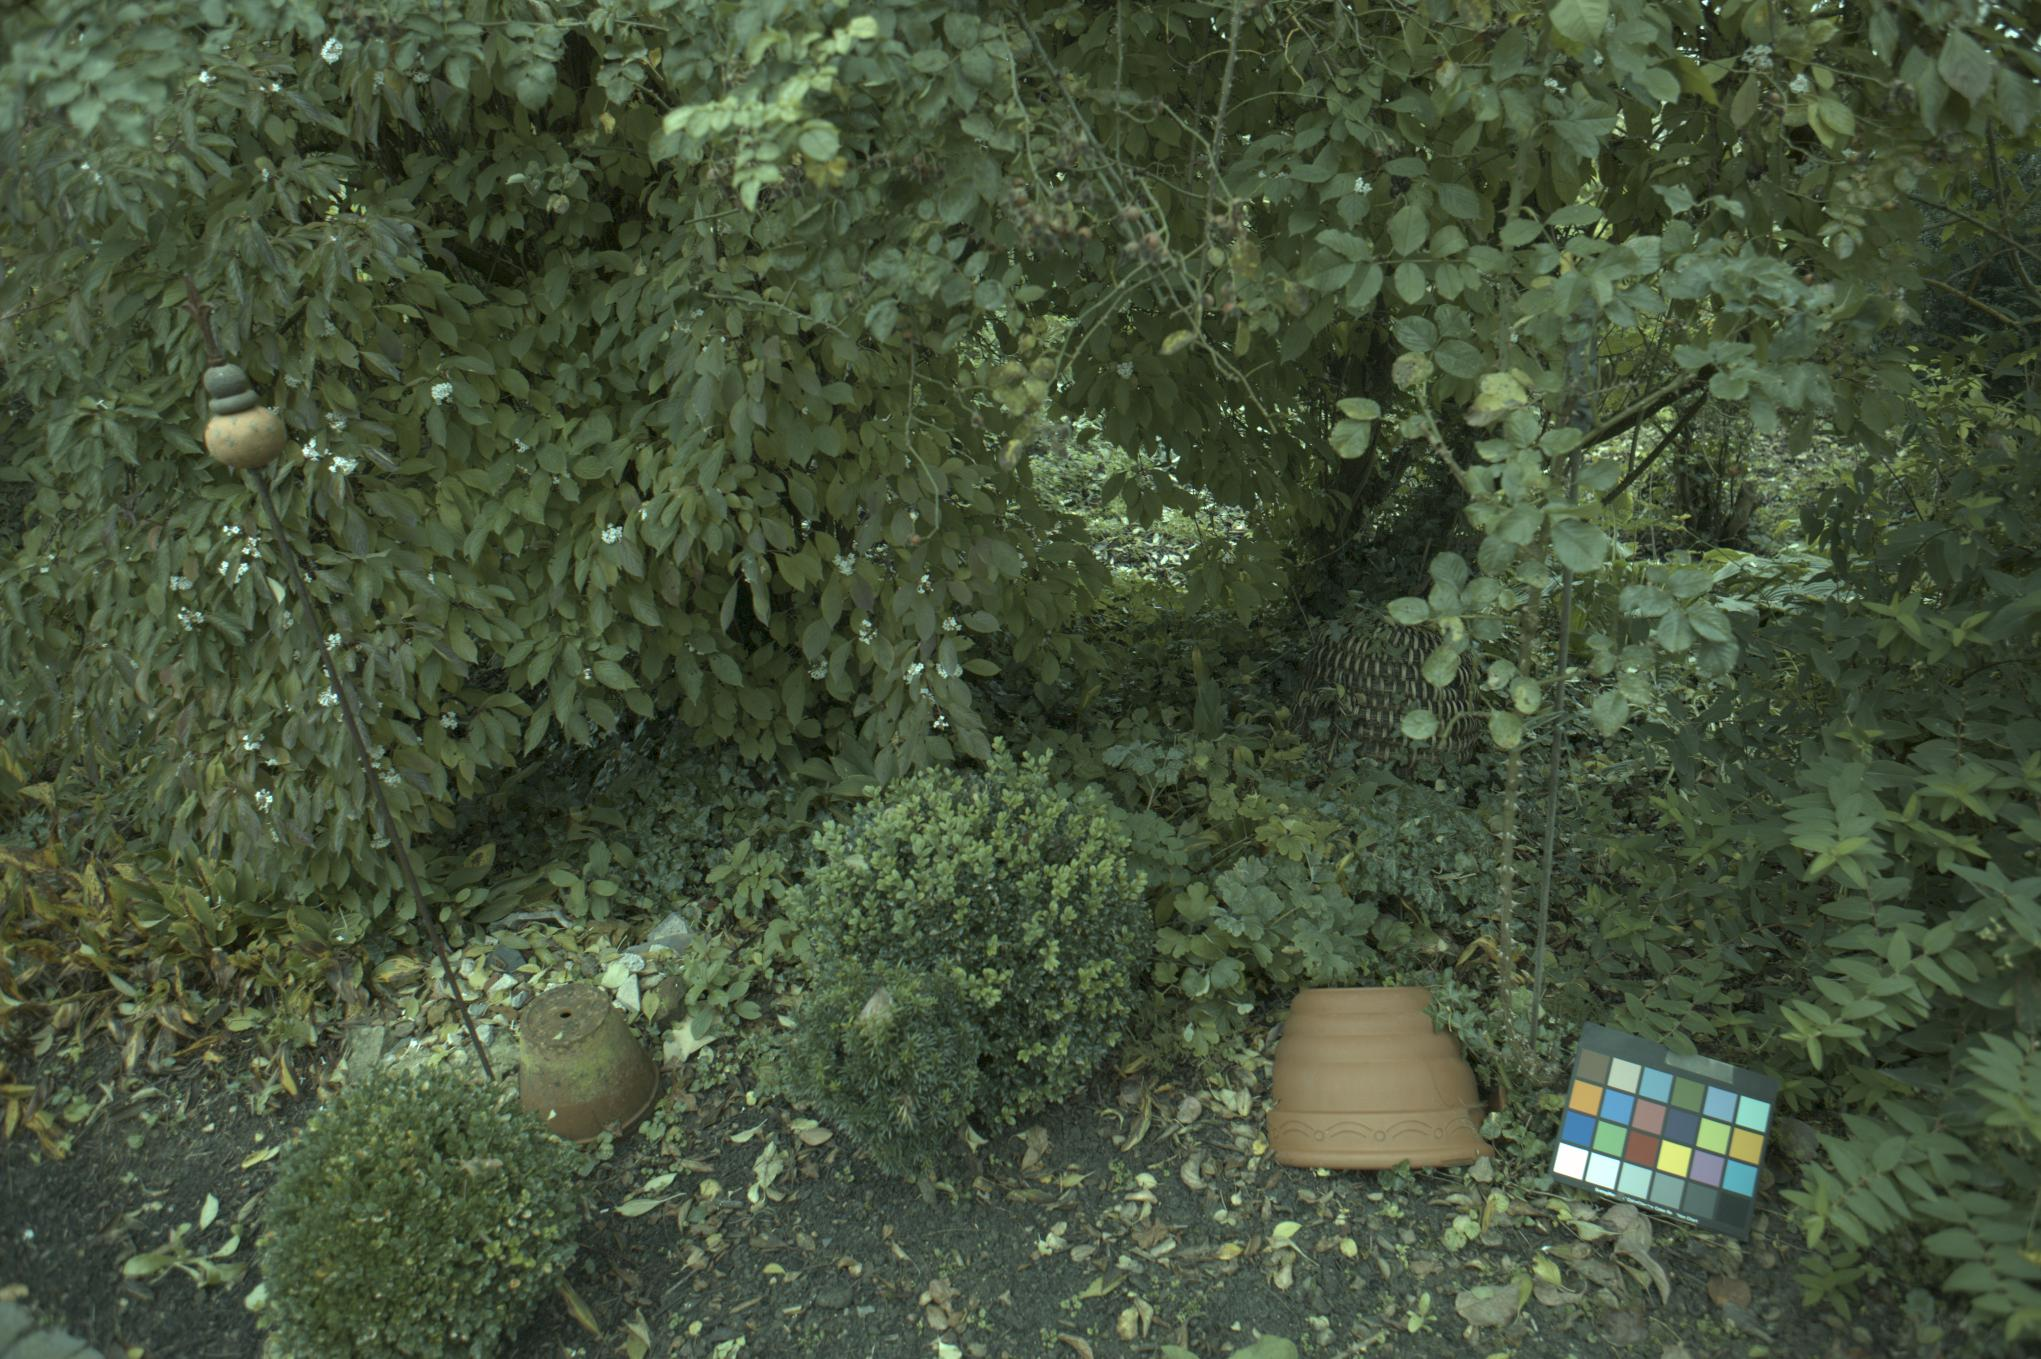
\includegraphics[height=15em]{code/inputs/cc/ex3.jpg}
	\includegraphics[height=15em]{code/outputs/prob2a_3.png}
	  \caption{balance2a-3}
\end{figure*}
\par

\spart{b}
white balance(2), in each Figure the first image is the one from part(a)

\begin{figure*}[h!]
  \centering
  	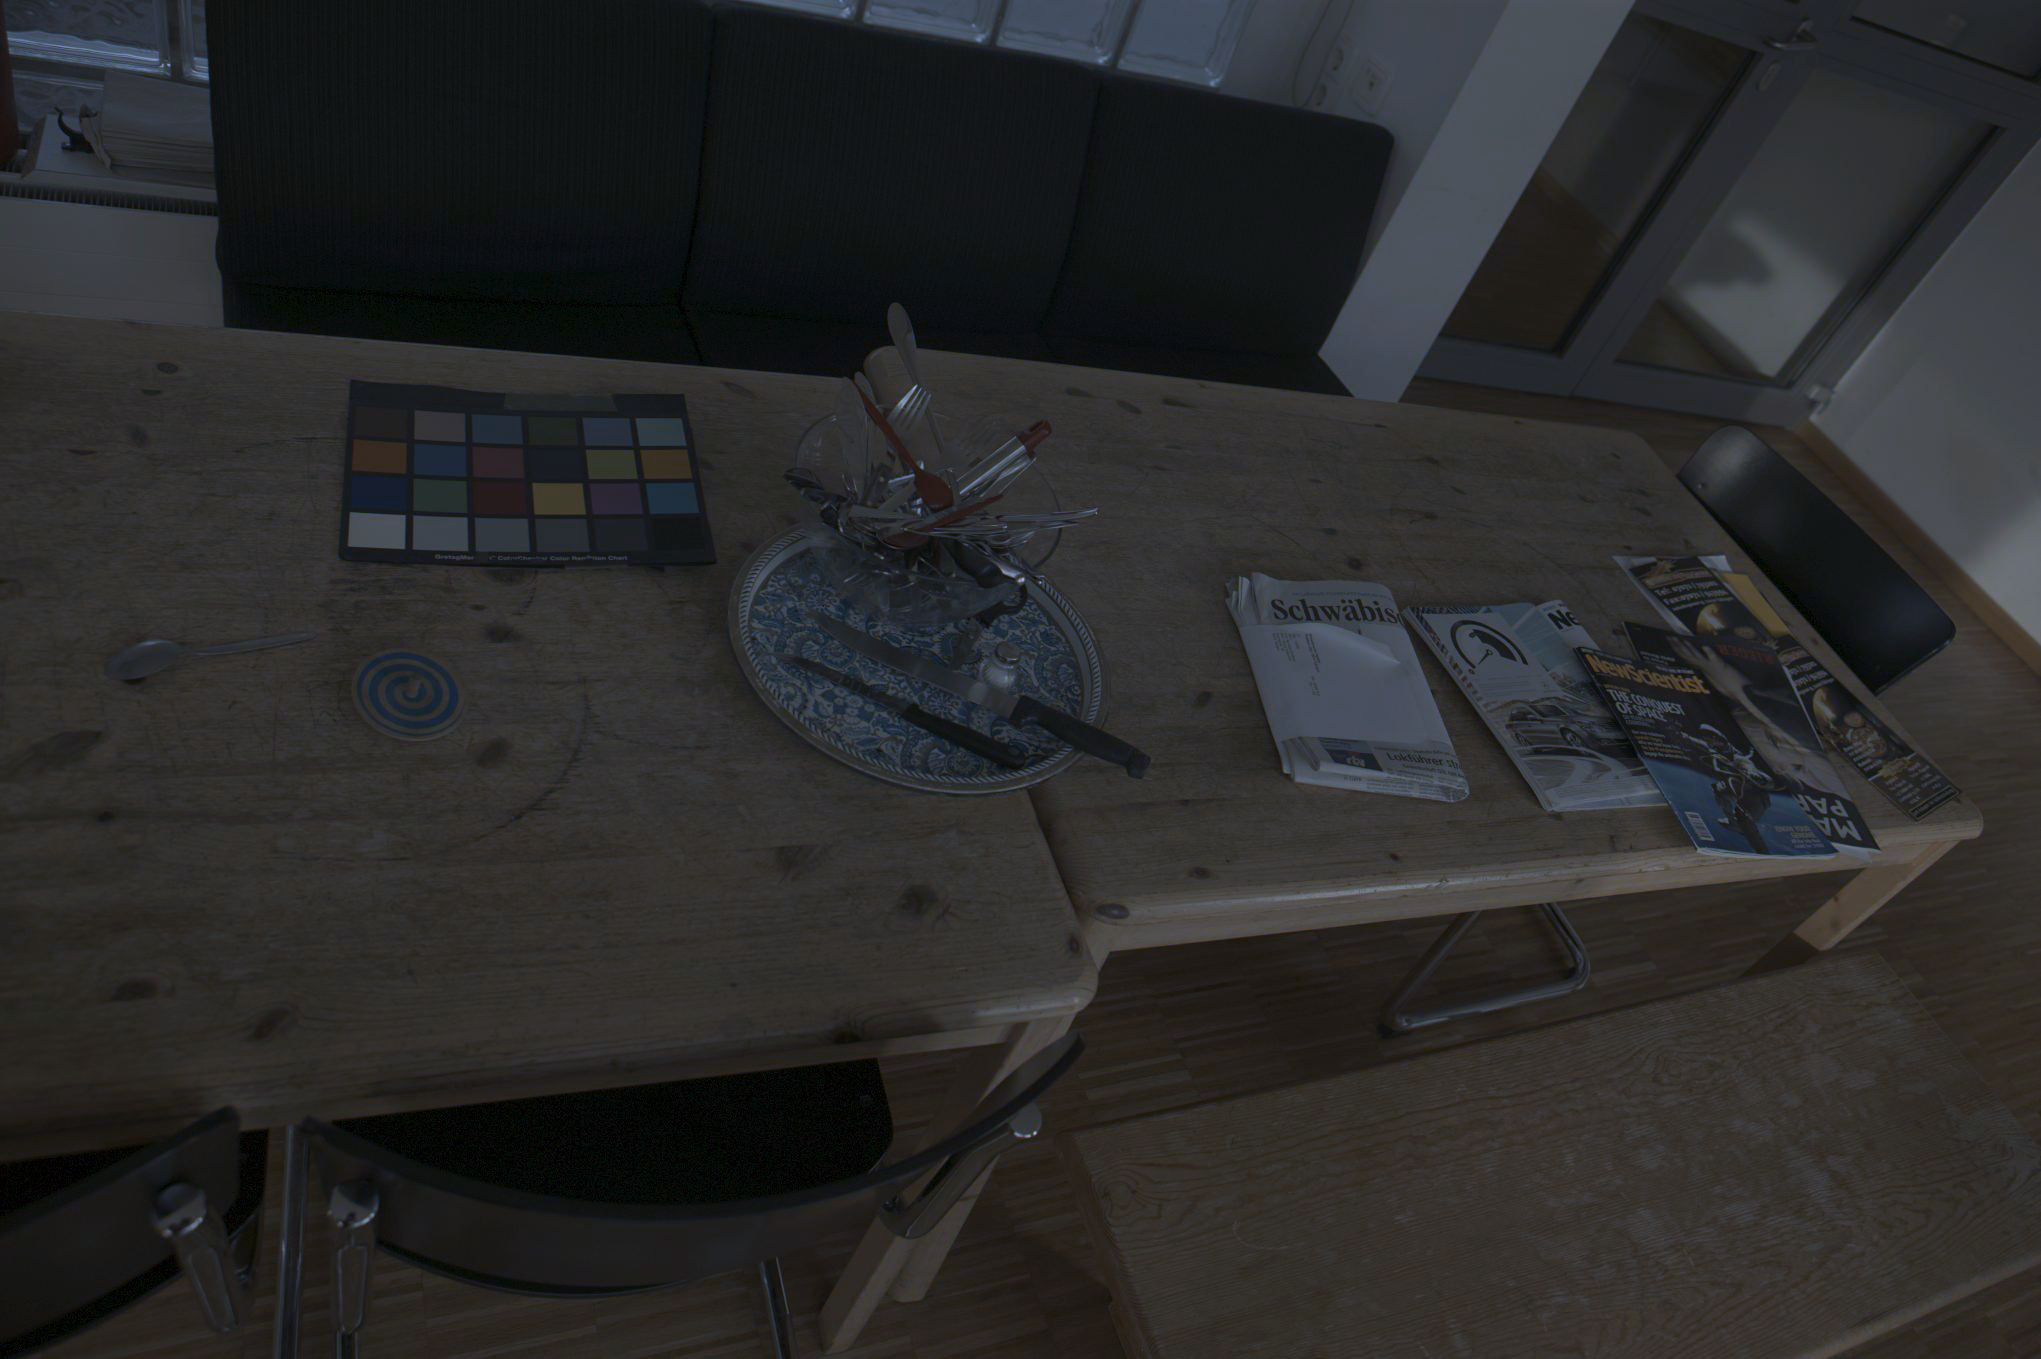
\includegraphics[height=15em]{code/outputs/prob2a_1.png}
	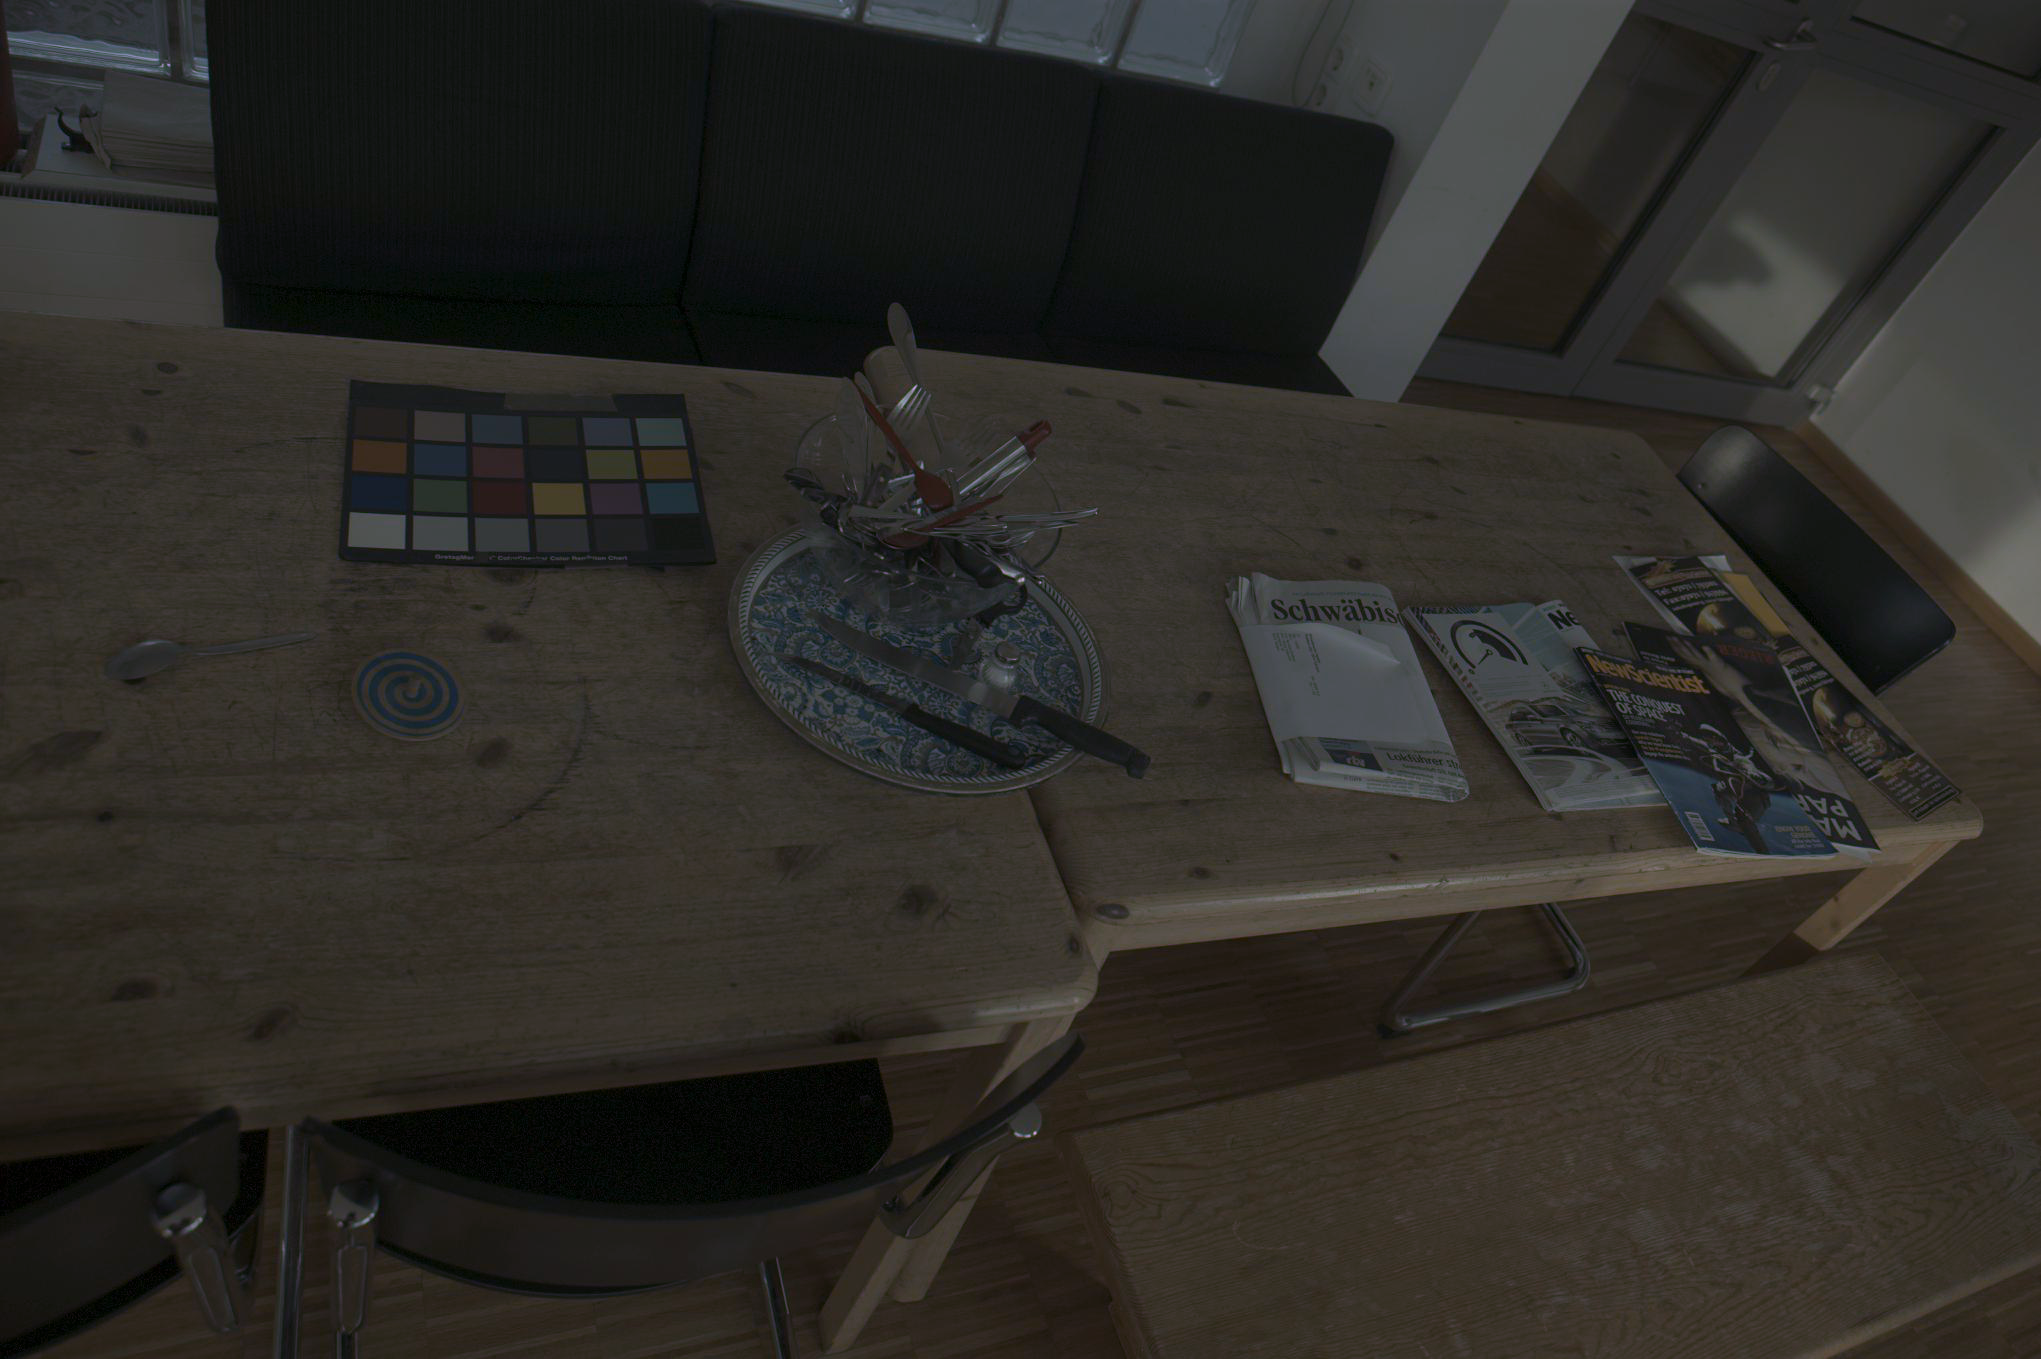
\includegraphics[height=15em]{code/outputs/prob2b_1.png}
	  \caption{balance2b-1}
\end{figure*}

\begin{figure*}[h!]
  \centering
  	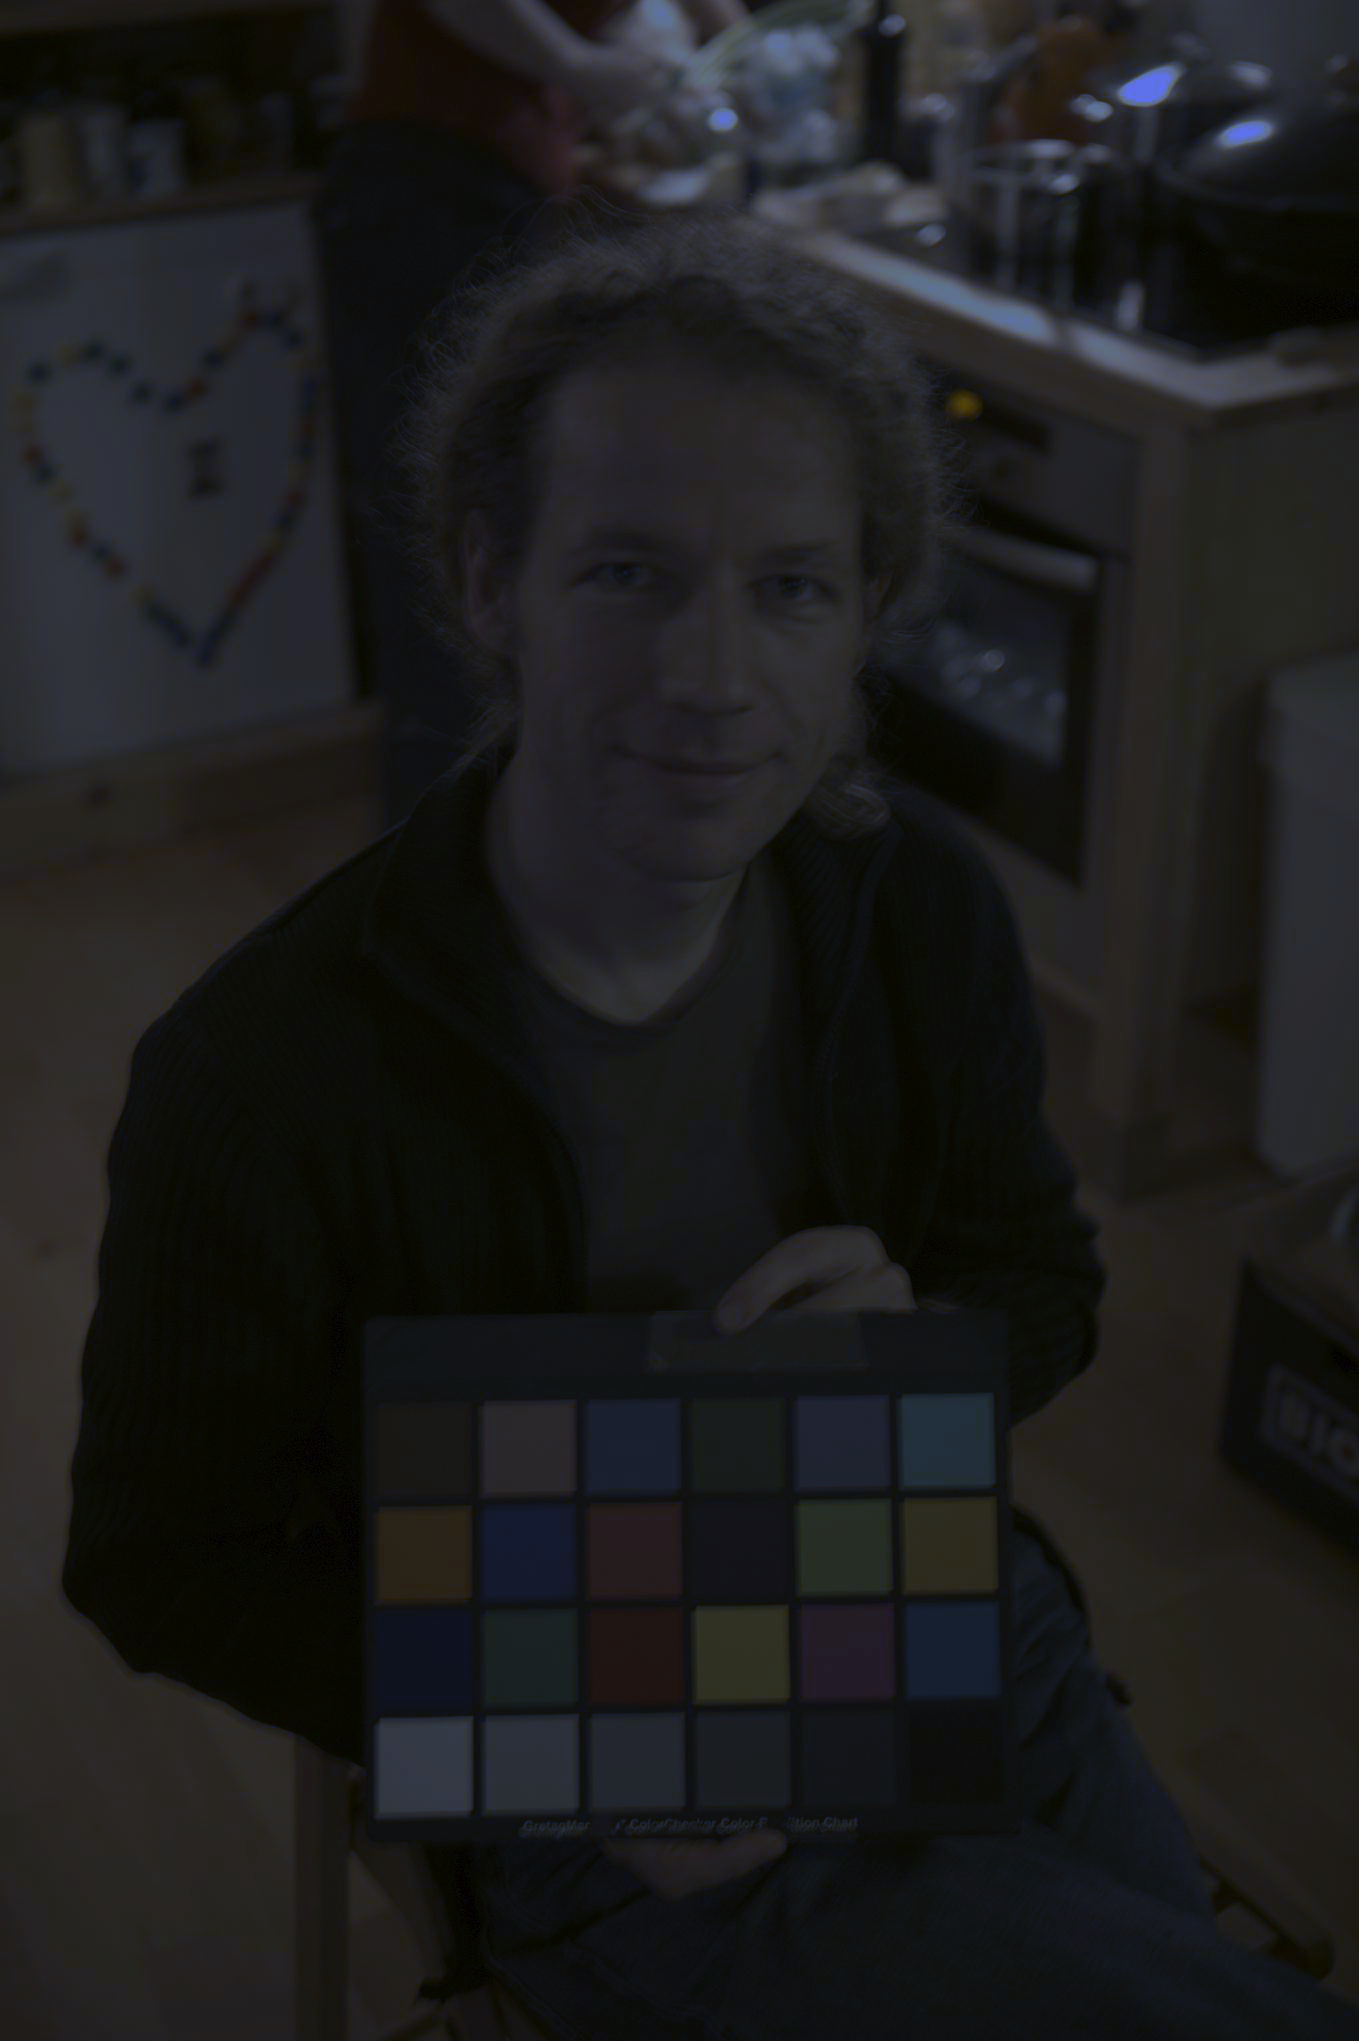
\includegraphics[height=20em]{code/outputs/prob2a_2.png}
	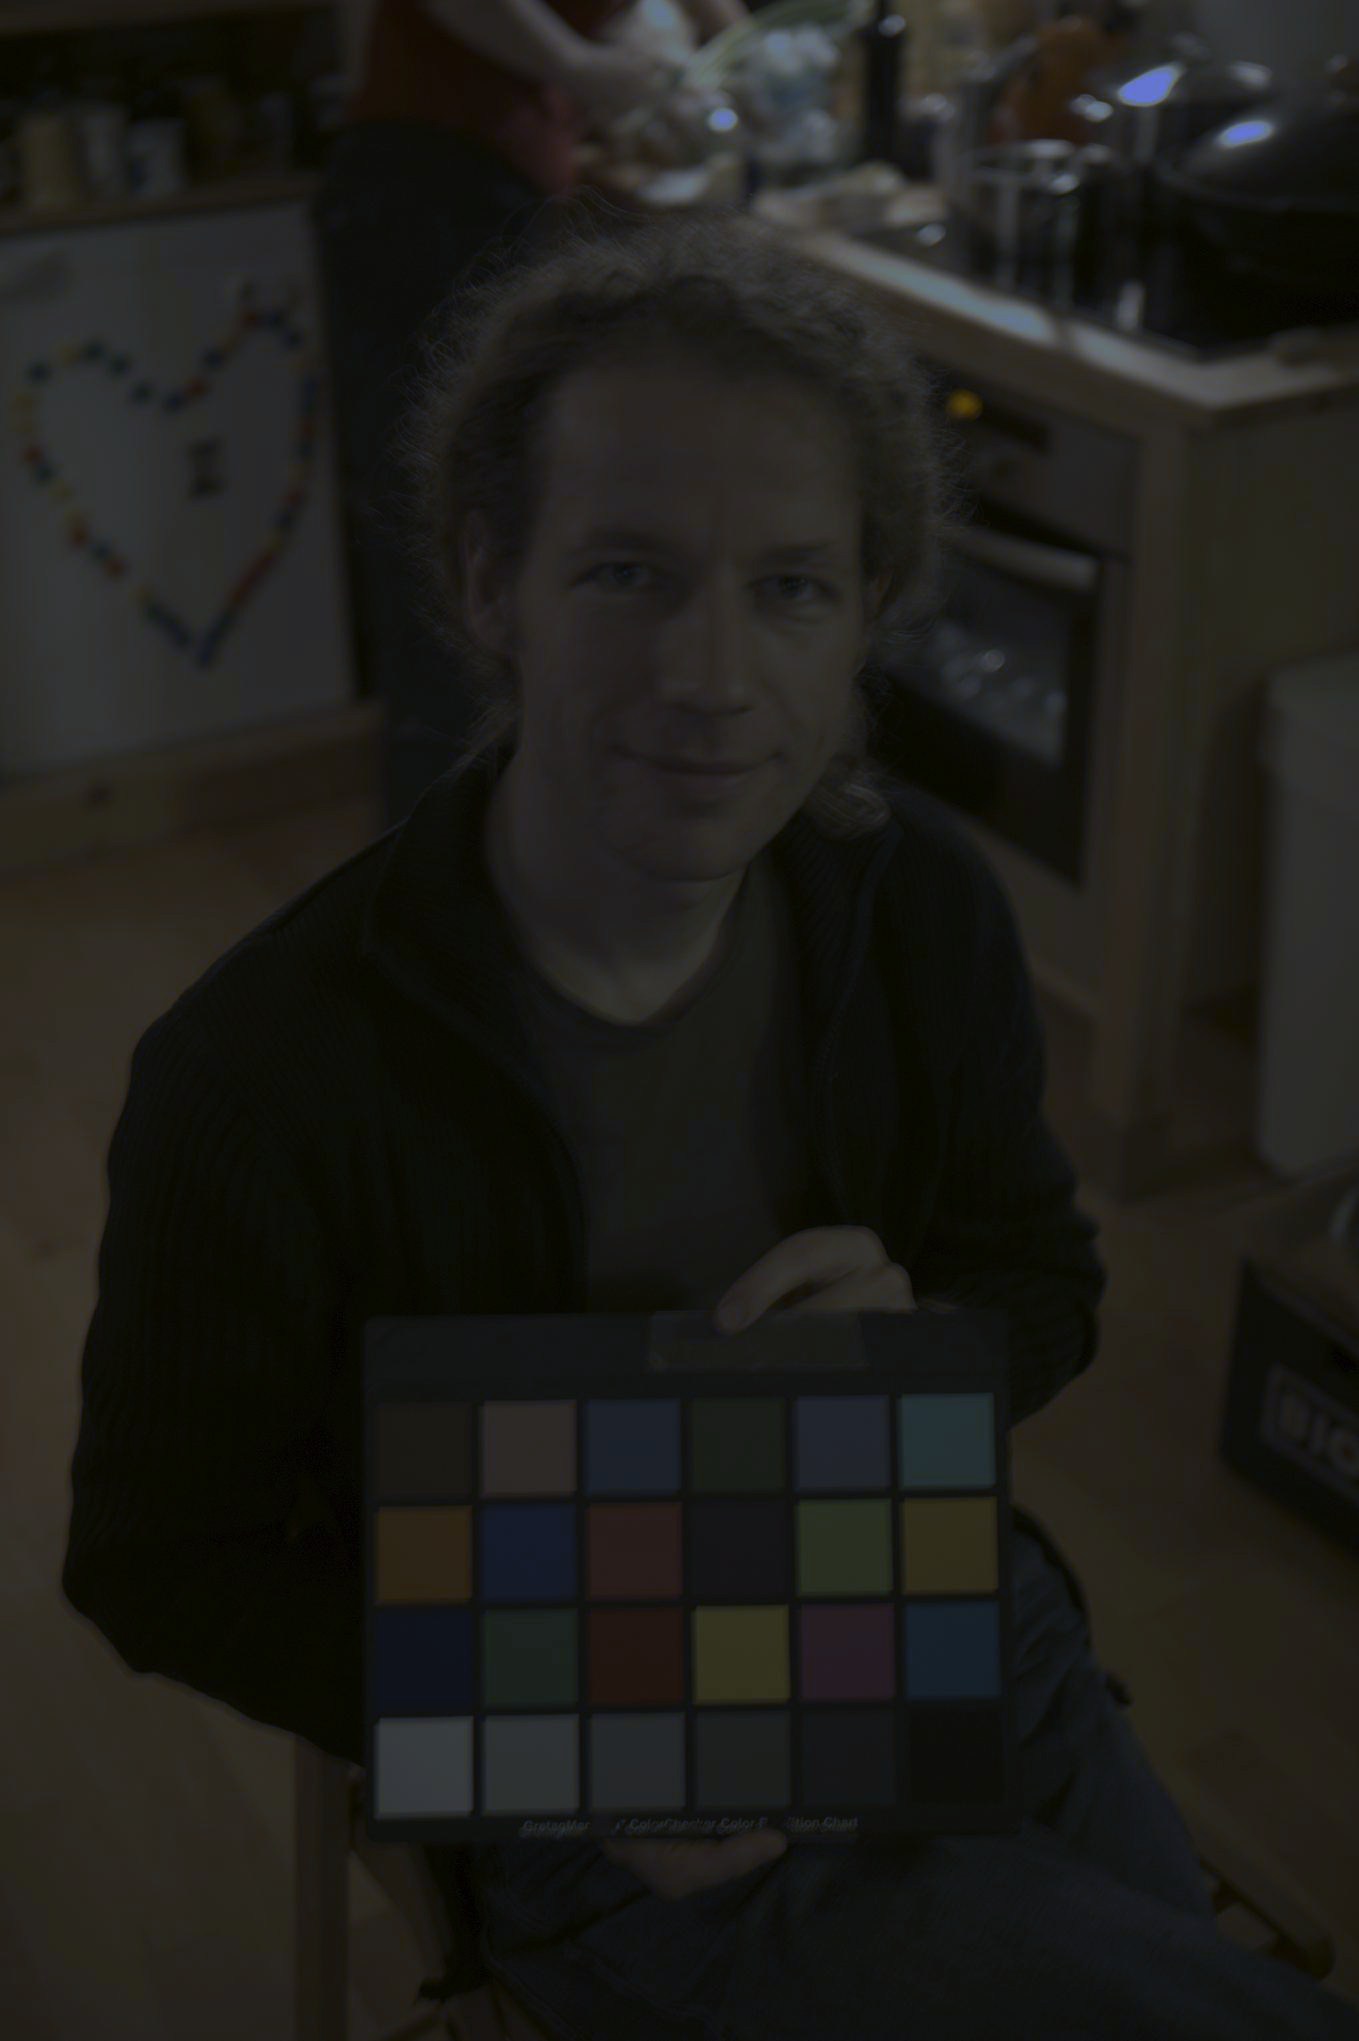
\includegraphics[height=20em]{code/outputs/prob2b_2.png}
	  \caption{balance2b-2}
\end{figure*}

\begin{figure*}[h!]
  \centering
  	\includegraphics[height=20em]{code/outputs/prob2a_3.png}
	\includegraphics[height=20em]{code/outputs/prob2b_3.png}
	  \caption{balance2b-3}
\end{figure*}

\solution{3}
\spart{a}
image of normals
\begin{figure*}[h!]
  \centering
  	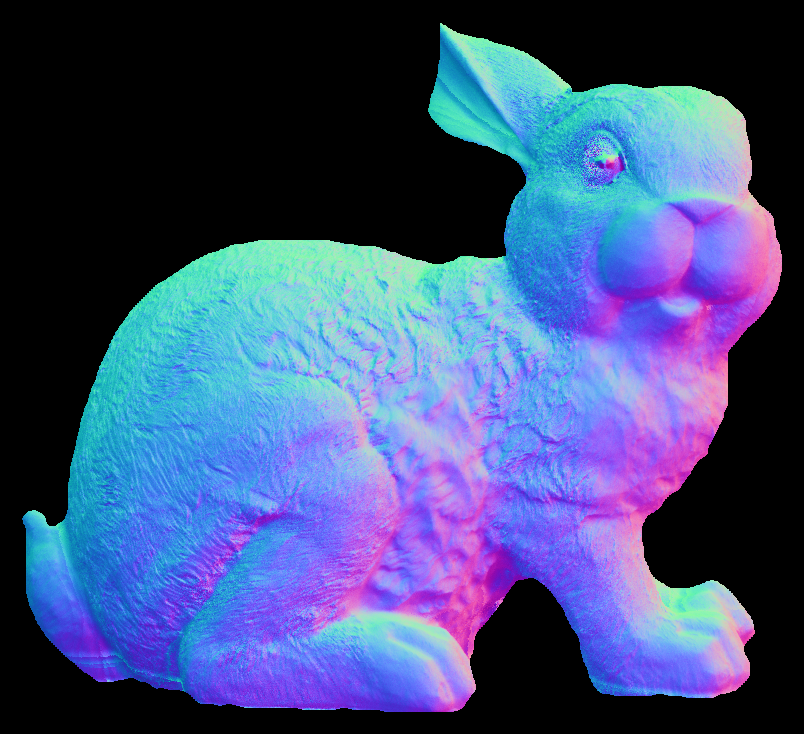
\includegraphics[height=20em]{code/outputs/prob3_nrm.png}
	  \caption{normals}
\end{figure*}

\spart{b}
image of the surface color $albedos$
\begin{figure*}[h!]
  \centering
  	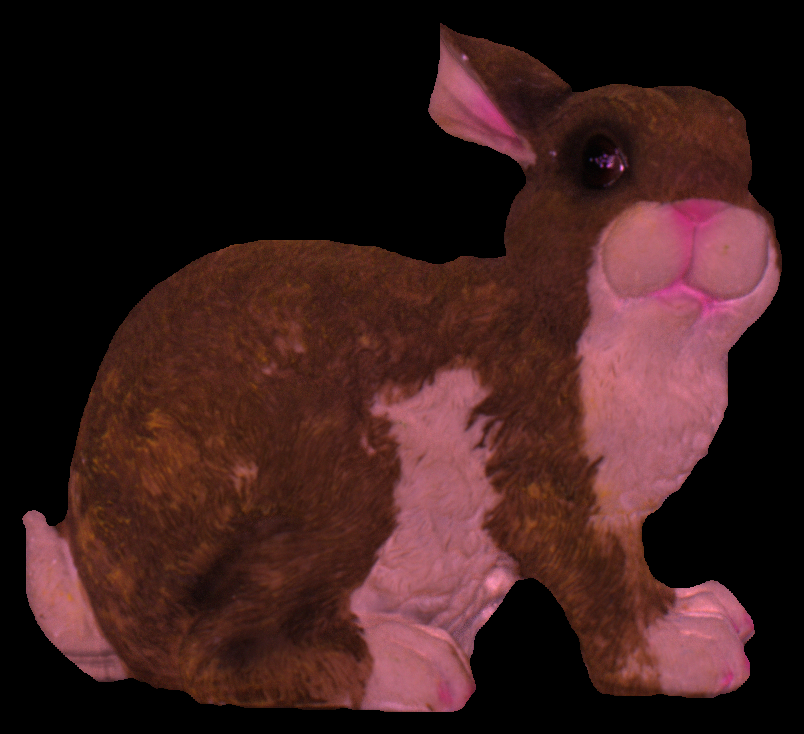
\includegraphics[height=20em]{code/outputs/prob3_alb.png}
	  \caption{albedos}
\end{figure*}

\solution{4}
Depth map by using Frankot-Chellappa method
\begin{figure*}[h!]
  \centering
  	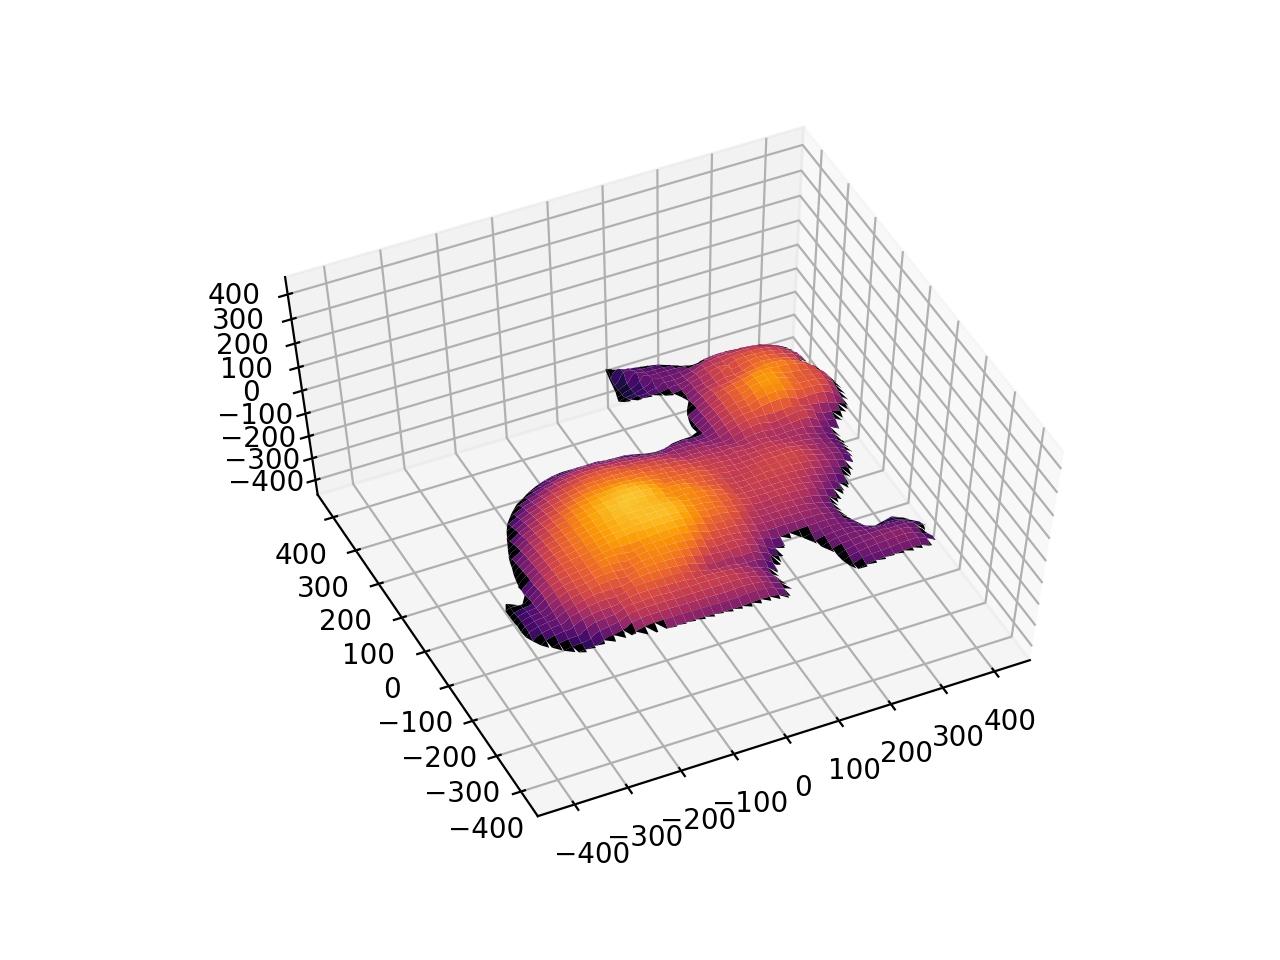
\includegraphics[height=40em]{code/outputs/prob4-1.png}
	  \caption{depth map}
\end{figure*}

\solution{5}
Depth map by using conjugate gradient method
\begin{figure*}[h!]
  \centering
  	
\includegraphics[height=40em]{code/outputs/prob5.png}
	  \caption{depth map}
\end{figure*}


\info

This problem set took approximately 30 hours of effort.


I discussed this problem set with:
\begin{itemize}
\item Sijia Wang
\item Jiarui Xing
\end{itemize}


% Note that you might have to escape some special symbols in URLS like \_
I also got hints from the following sources:
\begin{itemize}
\item lecture ppts
\end{itemize}

\end{document}
